\section{Introduction}
\label{sec:introduction}

\providecommand{\introchange}[1]{#1}
\providecommand{\structurechange}[1]{#1}
\providecommand{\localexecchange}[1]{#1}

Heterogeneous multi-manipulator systems must maintain a consistent task
interpretation while complementary robots execute concurrently in a changing
workspace. Figure~\ref{fig:scenario} instantiates this problem with a conveyor
and three task-relevant semantic events. Language- and vision-language-based
grounding~\cite{huang2023inner,liang2023code,rana2023sayplan} does not expose
team capability constraints or
responsibility interfaces; independent agents can therefore maintain
incompatible task views. The challenge is to
establish one capability-aware semantic authority across robots and revise only
the semantics invalidated by a new instruction, disturbance, or verified
failure while local controllers remain responsive to continuous scene
evolution. We propose RoSC, a role-shared semantic coordination framework with
an event-driven selective update that follows event detection $\rightarrow$
affected-scope selection $\rightarrow$ semantic-state revision $\rightarrow$
continued dispatch from a consistent frontier. Simulation baselines, failure
analysis, and mechanism ablations test these mechanisms, while hardware trials
check the same update sequence during physical execution.

\begin{figure}[t]
    \centering
    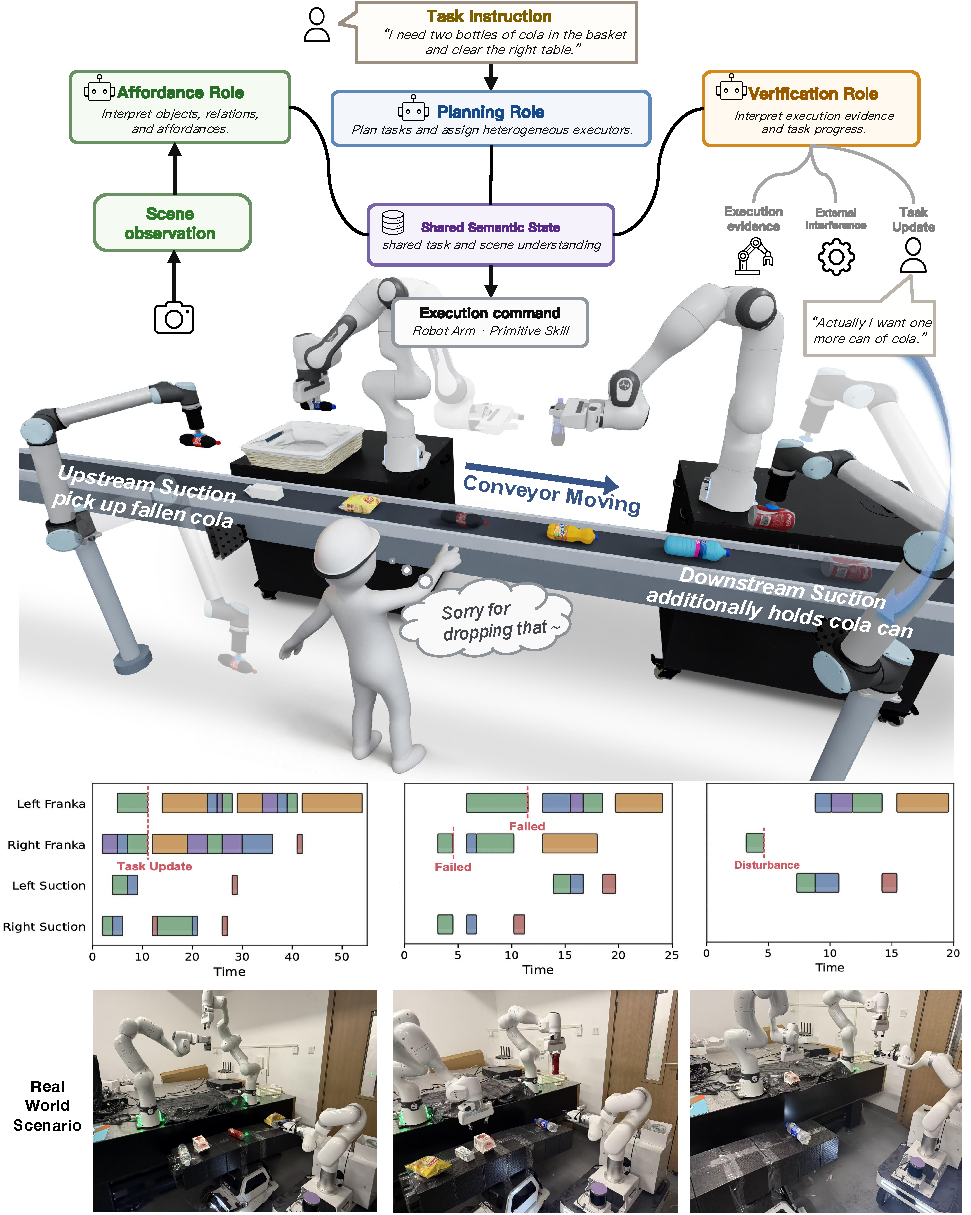
\includegraphics[width=\columnwidth]{figures/figure1_final_lowercase.pdf}
    \caption{The shared semantic state coordinates three roles while preserving
    local execution. \textbf{Top:} framework and simulated conveyor workspace;
    \textbf{Middle:} event Gantt charts; \textbf{Bottom left:} normal hardware
    execution; \textbf{Bottom middle:} hardware task update; \textbf{Bottom
    right:} hardware external disturbance.}
    \label{fig:scenario}
\end{figure}

\begin{figure*}[!t]
  \centering
  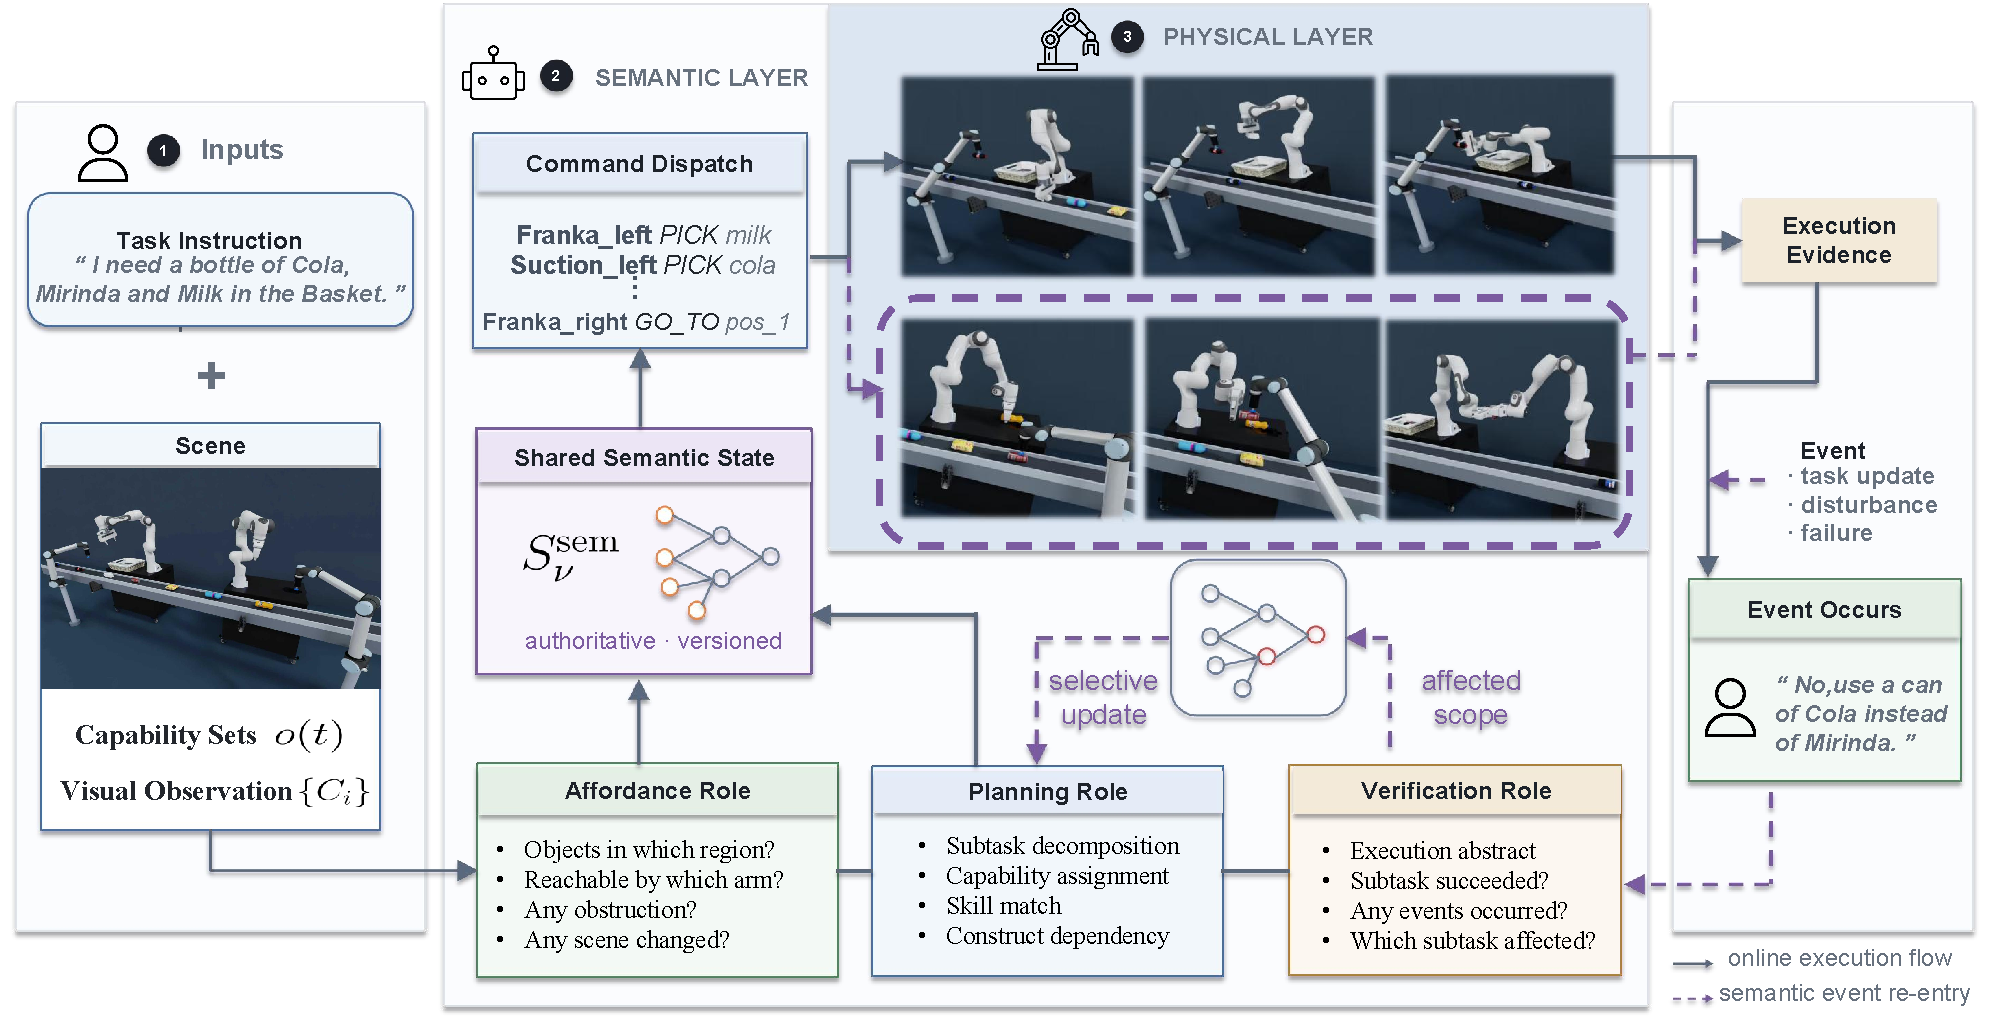
\includegraphics[width=0.96\textwidth]{figures/figure2.pdf}
  \caption{Role-shared coordination links semantic decisions to physical
  execution. Affordance evaluates scene feasibility; planning decomposes and
  assigns subtasks, skills, and dependencies; verification abstracts execution
  evidence, checks outcomes and events, and identifies affected subtasks. Solid
  and dashed arrows denote online execution and selective event updates.}
  \label{fig:method_overview}
\end{figure*}

\subsection{Related Work}
\label{sec:related_work}
\providecommand{\finalchange}[1]{#1}
\providecommand{\localexecchange}[1]{#1}

Language-guided grounding methods translate natural-language instructions into
spatial representations, executable programs, or scene-grounded task
plans~\cite{huang2023inner,liang2023code,rana2023sayplan,
huang2023voxposer}. Building on these capabilities, LLM-based multi-robot
frameworks adopt different coordination structures: RoCo uses inter-robot
dialogue; COHERENT relies on centralized proposals and execution feedback;
MALLVI reactivates specialized agents when needed; and CoMuRoS and DEXTER-LLM
revise tasks or assignments in response to events~\cite{
mandi2024roco,liu2025coherent,taji2026mallvi,
borate2026comuros,zhu2025dexter}. Other systems explicitly incorporate
capability-aware coalitions, dependency-based task allocation, or separate
planning, manipulation, and verification agents~\cite{
kannan2024smartllm,obata2025lipllm,he2026closedloop}. Collectively, these
methods establish effective mechanisms for grounding, agent interaction, and
task revision, but they do not explicitly organize ownership of the distinct
semantic components that must remain consistent as multiple heterogeneous
manipulators execute concurrently. RoSC addresses this issue by maintaining
the authoritative shared state and assigning responsibility
to the affordance, planning, and verification
roles, respectively. When a discrete semantic event occurs, these roles
identify its dependency-closed affected scope and reconstruct only the
invalidated subgraph, while preserving unaffected valid execution and leaving
continuous physical adaptation to the local controllers.


Dynamic manipulation supports tracked or reactive grasping and visual
servoing~\cite{marturi2019dynamic,maranci2026reactive,liu2023target,
haviland2020finalphase}, allowing local controllers to continuously adapt
end-effector motion to moving targets and perception updates. Execution
monitoring and continual replanning further address runtime deviations by
detecting discrepancies between expected and observed outcomes and invoking
recovery or plan revision~\cite{pettersson2005execution,brenner2009continual,
levihn2013foresight,pezzato2023active}. These methods primarily focus on
maintaining physical feasibility, monitoring action execution, or revising a
plan after deviations. However, in heterogeneous multi-manipulator settings,
the resulting feedback may affect different parts of the team-level semantic
state: a new observation may change an object's affordance, a failed action may
invalidate its execution status and downstream dependencies, and a revised
instruction may alter only one task branch. RoSC explicitly separates these
responsibilities among affordance, verification, and planning roles. It uses
the shared semantic state to determine which information must be refreshed,
which subtasks are affected, and whether planning should be invoked, thereby
supporting event-scoped semantic revision while preserving unaffected valid
execution.


\subsection{Our Method}
\label{sec:our_method_intro}

Figure~\ref{fig:method_overview} shows the resulting framework. At task start,
the affordance role evaluates object regions, reachability, obstructions, and
scene changes to produce $\mathcal{F}$; the planning role decomposes the task,
matches skills and capabilities to manipulators, constructs $G$, and initializes
the versioned shared semantic state
$S_\nu^{\texttt{sem}}=(\gamma,G,\mathcal{F},z)$. The framework then selects the
verified executable frontier, constructs capability-valid commands, and
dispatches independent commands concurrently to the assigned manipulators.
After local execution, affordance refreshes $\mathcal{F}$ and verification
abstracts the evidence, checks the outcome, updates $z$, and detects events. For
an event, verification identifies $\mathcal{N}_k^{\texttt{aff}}$; planning
replans that subgraph while preserving valid work outside it, then dispatch
continues from the updated frontier. This restricted semantic update shortens
the response path and helps preserve opportunities as the scene evolves.

The main contribution of this work is twofold: (I) A role-shared semantic
coordination formulation is introduced for dynamic heterogeneous
multi-manipulator scenarios with continual physical changes, assigning explicit
responsibility to the affordance, planning, and verification roles; and (II) An
event-driven selective semantic update procedure is developed to efficiently
handle task updates, external disturbances, and execution failures while
preserving unaffected valid execution.
